\chapter{How to operate}



One day  $+$ means to add natural numbers, the next day 
polynomials, later matrices.  
You can even add colors ``Yellow=Blue+Green''. When you program 
you learn to add strings
\begin{center}
\begin{notebookin}
print "Algebra " + " is " + " computation"
\end{notebookin}
\begin{notebookout}
Algebra is computation
\end{notebookout}
\end{center}
The $+$ is in fact a variable stand in for what we call a \emph{binary operator}
or \emph{bi-valent operator}.  It takes in a pair, 
according to the grammar $\Box+\Box$.  The valence (the number of inputs) and the grammar 
of an operator comprise its  \emph{signature}.  

Unlike these notes, addition should only be used when it is grammatically 
correct e.g.\ \emph{infix} $2+3$ rather than \emph{prefix} $+,2,3$ or
\emph{postfix} $2,3,+$.  Think of this like any other language 
where there could be a dialect that evolves the operator's grammar and lexicon.
Famously HP calculators were postfix for some time to match engineering requirements.
It turns out humans will adapt to technology easier than technology adapting to humans.
A program to add two lists could get away with the following linguistic drift:
\begin{center}
\begin{notebookin}
cat [3,1,4] [1,5,9]
[3,1,4] + [1,5,9]
\end{notebookin}
\begin{notebookout}[2]
[3,1,4,1,5,9]
[4,6,13]
\end{notebookout}
\end{center}
Using \texttt{cat} reminded us to concatenate and avoided confusion with the later $+$ 
concept.  It was the better choice.
Challenge yourself to see both as addition and you will 
find addition everywhere. 

Since we are evolving, we may as well permit multiplication as a binary operator
symbol, changing the signature to $\Box \cdot \Box$, i.e. $2\cdot 4$; or
$\Box\Box$, e.g. $xy$.   Avoid $\Box\times \Box$, we need that symbol elsewhere.
These days composition $\Box\circ\Box$ is written as multiplication; so, you can
use that symbol however you like.  Addition is held to high standards in algebra
(that it will evolve into linear algebra).  So when you are considering a binary
operation with few if any good properties, use a multiplication inspired
notation instead.   






Valence 1, \emph{unary}, operators include the negative sign $-\Box$ to create 
$-2$.  The transpose of a matrix is a unary operator.  Programming languages add several others 
such as \lstinline{++i, --i} which are said to \emph{increment} 
or \emph{decrement} the counter i (change it by $\pm 1$).


We can combine binary and unary operators to make useful (and useless) ternary 
operators.  One of my favorite (but generally useless) ternary products multiplies $(2\times 3)$-matrices,
that is right, rectangles not squares.  The product goes like this:
\begin{align*}
    [A,B,C] & = AB^{\dagger}C
\end{align*}
where $B^{\dagger}$ is the transpose.  A more serious product comes up 
in symmetric matrices where we need what is called the \emph{Jordan Triple product}
\begin{align*}
    \{A,B,C\} & = \frac{1}{6}(ABC+CBA)
\end{align*}
This is part of an whole family of Jordan products including 
\begin{align*}
    A\bullet B & = \frac{1}{2}(AB+BA)\\
    \langle A_1,\ldots,A_{\ell}\rangle & = \frac{1}{\ell!}(A_1\cdots A_{\ell}+A_{\ell}\cdots A_1).
\end{align*}
Notice in all these case if $A_i=A_i^{\dagger}$ then $\langle A_1,\ldots,A_{\ell}\rangle=
\langle A_1,\ldots,A_{\ell}\rangle^{\dagger}$.  So these are products that explain how 
symmetric matrices behave, and if you know about quantum mechanics that means these 
are the products you can use on observable quantum events.\footnote{Pascual Jordan was a physicist inventing 
math for quantum mechanics, not be be confused with Camile Jordan of Jordan-Holder and Jordan Normal form fame.}

Stranger ternary products showup in places where we wish we had easier binary products 
to explain things.  For example in geometry at small dimensions (dimension 2) we do not always 
have coordinates to explain what makes some set of points into a line. So Marshall Hall 
decided why not make a line $\ell$ be described by a ternary operator
\[
    -\otimes-\oplus -
\]
This is just notation but put in a formula like $y=m\otimes x\oplus b$ and you start to imagine 
the result as an algebraic line.  With this ternary product he was able to associated every 
projective plane to coordinates in some ternary ring.  Once you have such a ternary ring you 
can go to work to see if it might actually decompose into two binary operations of multiplicaton 
and addition, e.g.\ by locating a ``one'' and a ``zero'' where $x=1\otimes x\oplus 0$.  Then 
you reverse the process and define $m\cdot x\defeq m\otimes x\oplus 0$ and $x+b\defeq 1\otimes x\oplus b$
to get a more familiar ring-like structure.

Programs also exploit a ternary (valence 3) operator:
\begin{center}
    \lstinline[language=Sava]{if (...) then (...) else (...)}
\end{center}
The words, while helpful, are unimportant.  Some programming languages 
replace them with symbols emphasizing their ``opperatorness'' 
\begin{center}
    \lstinline[language=Sava]{_?_:_}
\end{center}
Here for example is division with remainder of positive integers
\begin{center}
\begin{lstlisting}[language=Sava,mathescape]
div(m,n)=(m>=n)?(div(m-n,n)+(1,0)):(0,m)
\end{lstlisting}
\end{center}
Programs go further making operators with huge valence.
If you find that interesting look into \emph{variadic} operators to see how 
far this idea goes.


A number of subtle problems are 
mounting.  For example, we probably want a Boolean (true/false) to 
go in the the left-most spot of an if-then-else-, and we cannot compose 
just any two functions and get expected results.  We scale a vector on one side 
by not the other.  Grammar must be more than just $\Box\cdot \Box$.



\section{Higher order Operators}
Lets consider an operator 

Another operator takes a pair $A$ and $B$ of sets or more general types 
of data and creates ordered pairs or disjoint unions.
\begin{gather}
    \tag{$\form{\times}$}
    \frac{A,B:Type}{A\times B:Type}\\
    \tag{$\intro{\times}$}
    \frac{a:A\quad b:B}{(a,b):A\times B}\\
    \tag{$\elim{\times}$}
    \frac{x:A\times B}{\pi_A(x):A}\qquad 
    \frac{x:A\times B}{\pi_B(x):B}\\
    \tag{$\comp{\times}$}
    \frac{a:A\quad b:B}{\pi_A(a,b)\defeq a}
    \qquad
    \frac{a:A\quad b:B}{\pi_B(a,b)\defeq b}
\end{gather}
In code you may encounter this as \lstinline{Pair[A,B]} or 
as \lstinline{(A,B)}.

\begin{lstlisting}[language=Hidris]
Either A B = Left (a:A) | Right (b:B)

apply (f:A->C, g:B->C, x:Either[A,B]) : C =
  match x with 
    Left a => f(a)
    Right b => g(b)
\end{lstlisting}
A special case of the disjoint union operator is to extend a type by 
one term:
\begin{align*}
    A^? \defeq A\sqcup \{*\}.
\end{align*}
It is said that $x:A^?$ is ``maybe an A'', or ``optionally A''.
In code you will find these written out this way.
\begin{lstlisting}[language=Hidris]
Maybe A = Just (a:A) | None
\end{lstlisting}
\begin{lstlisting}[language=Sava]
class Option[A]
    case Some(a:A) extends Option[A]
    case None extends Options[All]    
sealed  // You cannot add to these cases
\end{lstlisting}


A number of subtle problems are 
mounting.  For example, we probably want a Boolean (true/false) to 
go in the the left-most spot of an if-then-else-, and we cannot compose 
just any two functions and get expected results.  We scale a vector on one side 
by not the other.  Grammar must be more than just $\Box\cdot \Box$.

\chapter{Grammar school}

\begin{quote}
``... small number
of symbols and their grammar are enough to capture the huge
variety of equations...''
\end{quote}

Ask yourself how you know what to do when asked to  
calculate $7(7+3)^2$.  Parenthesis, Exponents, Multiplication, 
Division, Addition, Subtraction (PEMDAS) correct?  
Whether obvious or not, this is parsing grammar.  We can make this 
visual with a \emph{parse tree}.
\begin{center}
    \begin{tikzpicture}[yscale=0.75]
        \node (f) at (0,0) {$7(7+3)^2$};
        \node[below of=f,scale=0.75] {$\times$};
        \node (x1) at (-1,-2) {$7$};
        \node (sqrt1) at (1,-2) {$(7+3)^{2}$}; 
        % \node[below of=sqrt1,scale=0.75] {$\circ$};
        \node (su) at (1.5,-3) {\textasciicircum $2$};
        \node (u) at (1,-4) {$7+3$};
        \node (x2) at (0,-6) {$7$};
        \node[below of=u,scale=0.75] {$+$};
        \node (three) at (2,-6) {$3$};
        % \node (x3) at (0,-8) {$x$};
        % \node (x4) at (2,-8) {$x$};
        % \node[below of=x2,scale=0.75] {$\times$};

        \draw[-] (f) -- (x1);
        \draw[-] (f) -- (sqrt1);
        % \draw[-] (sqrt1) -- (su);
        \draw[-] (sqrt1) -- (u);
        \draw[-] (u) -- (x2);
        \draw[-] (u) -- (three);
        % \draw[-] (x2) -- (x3);
        % \draw[-] (x2) -- (x4);

    \end{tikzpicture}
    ~
    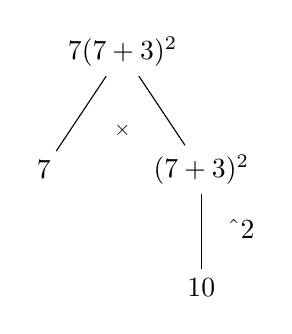
\begin{tikzpicture}[yscale=0.75]
        \node (f) at (0,0) {$7(7+3)^2$};
        \node[below of=f,scale=0.75] {$\times$};
        \node (x1) at (-1,-2) {$7$};
        \node (sqrt1) at (1,-2) {$(7+3)^{2}$}; 
        % \node[below of=sqrt1,scale=0.75] {$\circ$};
        \node (su) at (1.5,-3) {\textasciicircum $2$};
        \node (u) at (1,-4) {$10$};

        \draw[-] (f) -- (x1);
        \draw[-] (f) -- (sqrt1);
        % \draw[-] (sqrt1) -- (su);
        \draw[-] (sqrt1) -- (u);

    \end{tikzpicture}
    ~
    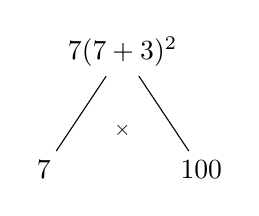
\begin{tikzpicture}[yscale=0.75]
        \node (f) at (0,0) {$7(7+3)^2$};
        \node[below of=f,scale=0.75] {$\times$};
        \node (x1) at (-1,-2) {$7$};
        \node (sqrt1) at (1,-2) {$100$}; 

        \draw[-] (f) -- (x1);
        \draw[-] (f) -- (sqrt1);

    \end{tikzpicture}
    ~
    $700$
\end{center}
We can read the tree like step-by-step instructions.  Start at the leaves and join
them by whatever operation is displayed on adjacent branches.
We start at the bottom with $7,3$, and join them as $7+3$ (computing $10$),
then the next step is to square (now $100$), then multiply by $7$, we reach $700$.
% Step-by-step?  Why not call it induction.
% Starting at the top, apply individualized 
% rules for each step.  Substitute in a product $MN[x\defeq 7]$ you compute 
% $M[x\defeq 7]N[x\defeq 7]$,
% sometimes denoted by a ``leads to'' relation $\leadsto$. So,
% with $M+N$ we can write,
% \[
%     (M+N)[x\defeq 7]\leadsto M[x\defeq 7]+N[x\defeq 7]
% \]
% At the end we finish off with rules like $3[x\defeq 7]\leadsto 3$ and $x[x\defeq 7]\leadsto 7$.
% If we use $x\defeq 3$ or $x\defeq t$ we use the same procedure.

You may have been taught induction through stories of falling 
dominos.  Good.  But what if induction was more like climbing, 
and the domino illustration was bottling up the experience
of climbing stairs?  Surely its more fun to climb trees and mountains.
Climbing can go up (induct) or down (recurse), but of course I drew the 
tree upside-down; so, the metaphor must be rotated.
My goal is to turn all of your views on induction on their head.
There are many inductions, one for each free algebra, but that's the forest 
and we should look first at some more trees.

\begin{quote}
    \textbf{Complex inductions can be specified by grammar.}
\end{quote}
\section{Grammar}
Climbing could find many routes, even go in cycles, but 
evaluating a formula was a precise algorithm without ambiguity.
The reason was that we had a tree.  Trees have unique paths between 
any two vertices. So if we start at the bottom we have a unique direction to 
reach the top.  Recursion on trees is so special it has a special name:
\emph{traversing} the tree.  

Parsing grammars in natural language is not always that
uniform.  English grammar may have cycles.
\begin{center}
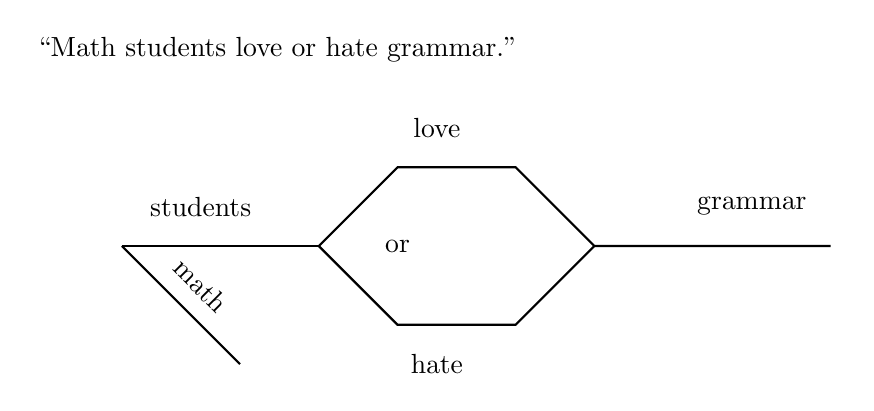
\begin{tikzpicture}
    \node[text width=4in] at (0,2) {``Math students love or hate grammar.''};
    \node at (-3,0) {students};
    \node[rotate=-45] at (-3,-1) {math};
    \node at (-0.5,-0.5) {or};
    \node at (0,1) {love};
    \node at (0,-2) {hate};
    \node at (4,0) {grammar};

    \draw[thick] (-4,-0.5) -- ++(2.5,0);
    \draw[thick] (-4,-0.5) -- ++(1.5,-1.5);
    \draw[thick] (-1.5,-0.5) -- ++(1,1) -- ++(1.5,0) -- ++(1,-1) -- ++(3,0);
    \draw[thick] (-1.5,-0.5) -- ++(1,-1) -- ++(1.5,0) -- ++(1,1);

\end{tikzpicture}
\end{center}
In mathematics two paths to the same place are said to be a relation, 
they are related.  So systems that have no cycles, i.e.\ trees, are 
free of relations, or simply \emph{free}.  What is free in this case 
is the grammar we used for arithmetic formulas.  That is not be confused 
with saying that we couldn't some how rewrite a formula to mean the same thing.
For example $7(7+3)(7+3)$ is a different formula with the same result.
But if we diagrammed that formula as parse tree it would quite different,
and it would not have a cycle.

\index{context-free}
That we got a tree in math formulas means we have a rather boring grammar, 
what Chompsky's \emph{Syntactic Structure} calls
\emph{context-free} grammars.\footnote{
    If an algebraist starts a talk with a story that ``...It was thought  all natural 
    languages were context-free until some obscure dialect in the alps or Africa was found...'', 
    then tune out until they return to equations.  
    Linguist never had such illusions. Even english is not context-free, read  James Higginbotham.} 
Don't be too disheartened.  Virtually every programming language has a 
context-free grammar and programs can communicate a lot of hefty ideas. 

% Induction in context-free grammars is to build ``up''
% taking fixed types of leaves and combining them with branches till we reach the root.
\index{langauge}
To specify a context-free grammar we specify the atoms of our language. For
natural numbers we can used digits $0,1,\ldots, 9$.  Then we write down patterns
of how to combine digits.  The separate cases are designated by the auxiliary
symbol `$|$' (which reads as ``or'').  Each rule is given a name called a
\emph{token} (or \emph{tag}) and denoted \lstinline{<Name>}. Since the Walrus
$\defeq$ is our assignment of variables, we use the ``astonished Walrus'' $::=$
as assignment of token rules. Listing~\ref{lst:nat-grammar} shows the grammar
for natural numbers as digits.
\begin{lstfloat}
\begin{lstlisting}[mathescape]
     <PosDig> ::= 1 | 2 | 3 | 4 | 5 | 6 | 7 | 8 | 9 
       <Nat>  ::= 0 | <PosDig> | <PosDig><Nat>
\end{lstlisting}
\caption{The grammar for natural numbers.}
\label{lst:nat-grammar}
\end{lstfloat}

The natural number grammar is said to \emph{accept} $0$ as a natural number,
written ``0:Nat''.  It also accepts 541:Nat and 10:Nat but it rejects ``01:Nat''
as that case does not exist as a production rule for any token in this grammar.

\begin{center}
    \begin{tikzpicture}
        \node at (-3.5,0) {\begin{tikzpicture}
            \node (10) at (0,0) {10:Nat};
            \node (1) at (-2,-2) {1:PosDig};
            \node (0n) at ( 2,-2) {0:Nat};
            \draw[thick] (0n) -- (10) -- (1);
            \node[below of=10,scale=0.75,text width=0.6in] {Nat case 3};
        \end{tikzpicture}};
        \node at (3.5,0) {\begin{tikzpicture}
            \node (01) at (0,0) {01:Nat};
            \node (1) at ( 2,-2) {1:PosDig};
            \node (0n) at (-2,-2) {0:Nat};
            \draw[thick,dashed] (0n) -- (10) -- (1);
            \node[below of=01,scale=0.75,text width=0.6in] {no case!};
        \end{tikzpicture}};
    \end{tikzpicture}
    \end{center}

Induction is to apply production rules, so it can
only ever deliver a sentence accepted by the grammar. The strings accepted by
our grammar are known as the  \emph{language} for that grammar.  They are the
source of one of the most important algebras out there, the free algebras.
        
Deciding to accept or reject is recursion, and so it may start with some string
using the alphabet but with the wrong grammar and reach a point of failure, or
it might get stuck trying to decide.  Context-free grammars fortunately never
get stuck, they do not even need a full strength computer to run (a push-down 
automata will do, like the chip you might need to run a microwave).
Yet Moore's law makes actual computers abundant so lets skip the microwave 
in favor of a general purpose program to parse.


\begin{lstfloat}
    \begin{lstlisting}[language=Hidris]
    posDigitize( token:Char):Option[PosDig] =
        match token with
        '1' => Some 1:PosDig;   '2' => Some 2:PosDig;   
        '3' => Some 3:PosDig;   '4' => Some 4:PosDig;   
        '5' => Some 5:PosDig;   '6' => Some 6:PosDig;
        '7' => Some 7:PosDig;   '8' => Some 8:PosDig;   
        '9' => Some 9:PosDig;
        _  => None
    
    digitize( stream:String ):Option[Digit] =
        match stream with 
            nil => None
            head::tail => 
                match head with 
                    '0' => match tail with 
                                nil => Some <0,0>:Nat
                                 _  => None
                     _ => match posDigitize(head) with 
                            Some (x:PosDig) => 
                                match digitize(tail) with 
                                    Some (y:Nat) => <(10^(y.digits)*x+y),1+y.digtis>:Nat
                                    None => None
                            None => Some (<x,1>:Nat)
    \end{lstlisting}
    \caption{Parsing}
    \end{lstfloat}
    
% Having a tree makes moving about the nodes a unique process, because trees 
% have a unique path between any to vertices.  So if we root the tree at the start 
% we have a unique path to get to the leaves, where we place the base cases.  
% Recursion on trees is so special it has its own name: \emph{traversing}.
% Of course, if we are doing one step at a time we still have choices: first go left, then go right, and 
% etc.  That is our next concern.



% \subsection{Vocabulary.}\index{production}\index{production!binary} The rules in
% the grammar are often described as \emph{production rules}.  For example,
% \lstinline{<Nat> ::= <PosDig><Nat>} produces a natural number by taking in a
% positive digit and a natural number.  We call it a \emph{binary} production
% because it takes two inputs.  We also call it \emph{heterogeneous} because it
% takes in data of different types.  (If all the inputs and outputs are of the
% same type we call the production \emph{homogeneous}.)  Some productions take in
% only one input, so-called \emph{unary}, such as squaring a number, or the first
% case of \lstinline{<Nat>} which takes in a digit and is said to \emph{promote}
% the term to a natural number.\footnote{Promote improves over the alternative
% \emph{coerce}, which in turn replaced the use of ``caste''---an all too casual
% allusions to a discriminator societal system.} Productions that require no
% preexisting data, such as the digits $0,\ldots,9$, are called \emph{nullary},
% \emph{atomic}, or \emph{terminal}. \index{nullary}\index{atomic}\index{terminal}

\begin{remark}
The symbols \lstinline{::=}, \lstinline{<Token>} and \lstinline{|} are 
Backus-Naur Form (BNF) notation, which is popular 
in computer science.  It is actually subject to its own gammar, admittedly 
basic and fixed in length.  But you can be forgiven for wondering if this is 
all circular reasoning.  When this occurs, mathematicians like to attach 
the word \emph{meta}, which means literally ``self-referential''.
So BNF would be called a \emph{meta-language}. Sometimes self-referential 
can be turned into paradoxes (Russell's paradox, G\"odel's Incompleteness,
Turing's Halting problem).  So you may worry.  But I suppose if you 
didn't believe in language, why would you be reading?\\
\end{remark}

All these ideas appear under different notation in 600 BC by Panini's rules of
Sanskrit grammar.  Good ideas get rediscovered; great ideas get reappropriated.



\begin{quote}
    \textbf{Context-free grammars parse into trees leading complex inductions 
    that are still follow a  unique path.}
\end{quote}

